\documentclass{beamer}

\usepackage[T1]{fontenc}
\usepackage[utf8]{inputenc}
\usepackage[english]{babel}
\usepackage{lmodern}
\usepackage{tikz}
\usetikzlibrary{positioning}

% Use Unipd as theme, with options:
% - pageofpages: define the separation symbol of the footer page of pages (e.g.: of, di, /, default: of)
% - logo: position another logo near the Unipd logo in the title page (e.g. department logo), passing the second logo path as option 
% Use the environment lastframe to add the endframe text
\usetheme[pageofpages=of]{Unipd}

\title{I - Neural Turing Machines}
\subtitle{Application to physical simulations}
\author[Lucia Fernandez Sanchez, Alexandra Perruchot-Triboulet Rodriguez, Samuel Chapuis]{L.~Fernandez Sanchez \and A.~Perruchot-Triboulet Rodriguez \and S.~Chapuis}

\date{\today}

% The next block of commands puts the table of contents at the beginning of each section and highlights the current section
\AtBeginSection[]
{
  \begin{frame}
    \frametitle{Table of Contents}
    \tableofcontents[currentsection]
  \end{frame}
}



\begin{document}

% Make the title page
\frame{\titlepage}


\section{From Navier--Stokes to Simplified PDEs}

% ===== Slide 1 =====
\begin{frame}{Navier Stokes to Simplified PDEs}
\small
\textcolor{red_unipd}{\Large Navier--Stokes (2D, incompressible)}

\vspace{0.6em}

\begin{alertblock}{Equation}
\[
\begin{cases}
\dfrac{\partial \mathbf{u}}{\partial t} 
+ (\mathbf{u}\!\cdot\!\nabla)\mathbf{u}
= -\nabla p + \nu\nabla^2 \mathbf{u},\\[4pt]
\nabla\!\cdot\!\mathbf{u} = 0
\end{cases}
\]
\end{alertblock}

\vfill

\begin{block}{Hypotheses}
Incompressible: \(\nabla\!\cdot\!\mathbf{u} = 0\). \quad
Viscous: \(\nu>0\). \quad
Free pressure: \(p(x,y,t)\).
\end{block}
\end{frame}


% ===== Slide 2 =====
\begin{frame}{Navier Stokes to Simplified PDEs}
\small
\textcolor{red_unipd}{\Large Euler (Inviscid Fluid)}

\vspace{0.6em}

\begin{alertblock}{Equation}
\[
\dfrac{\partial \mathbf{u}}{\partial t} 
+ (\mathbf{u}\!\cdot\!\nabla)\mathbf{u}
= -\nabla p
\]
\end{alertblock}

\vfill

\begin{block}{Hypotheses}
No viscosity: \(\nu = 0\). \quad
(Optional) Incompressible: \(\nabla\!\cdot\!\mathbf{u}=0\).
\end{block}
\end{frame}


% ===== Slide 3 =====
\begin{frame}{Navier Stokes to Simplified PDEs}
\small
\textcolor{red_unipd}{\Large Burgers (1D Advection–Diffusion)}

\vspace{0.6em}

\begin{alertblock}{Equation}
\[
\dfrac{\partial u}{\partial t} + u\dfrac{\partial u}{\partial x}
= \nu\dfrac{\partial^2 u}{\partial x^2}
\]
\end{alertblock}

\vfill

\begin{block}{Hypotheses}
\(\nabla p=\mathbf{0}\). \quad
1D reduction: \(\mathbf{u}=(u(x,t),0)\). \quad
Self-advection: \(u\,\partial_x u\).
\end{block}
\end{frame}


% ===== Slide 4 =====
\begin{frame}{Navier Stokes to Simplified PDEs}
\small
\textcolor{red_unipd}{\Large Heat / Diffusion Equation}

\vspace{0.6em}

\begin{alertblock}{Equation}
\[
\dfrac{\partial u}{\partial t} =
\alpha\,\dfrac{\partial^2 u}{\partial x^2}
\]
\end{alertblock}

\vfill

\begin{block}{Hypotheses}
No convection: \(u\,\partial_x u = 0\). \quad
Pure diffusion: \(\alpha>0\).
\end{block}
\end{frame}


% ===== Slide 5 =====
\begin{frame}{Navier Stokes to Simplified PDEs}
\small
\textcolor{red_unipd}{\Large Darcy (Steady, Elliptic Form)}

\vspace{0.6em}

\begin{alertblock}{Equation}
\[
\nabla\!\cdot\!\big(a(x)\nabla u(x)\big) = f(x)
\]
\end{alertblock}

\vfill

\begin{block}{Hypotheses}
Steady regime: \(\partial_t u = 0\). \quad
Heterogeneous medium: \(a(x)>0\). \quad
Source/sink: \(f(x)\).
\end{block}
\end{frame}



% ===== Slide 6 =====
\begin{frame}{Navier Stokes to Simplified PDEs}
\small
\textcolor{red_unipd}{\Large Summary of Relationships}

\centering
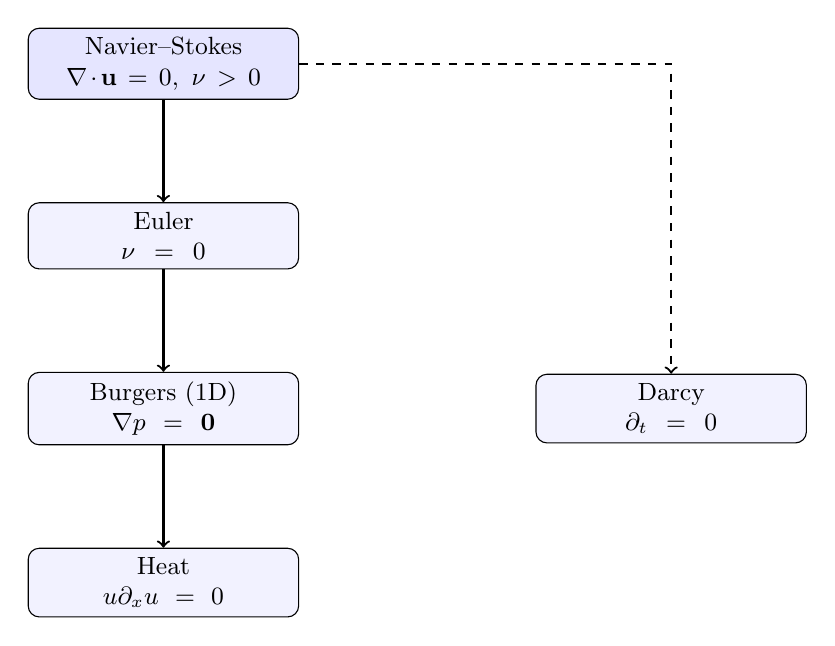
\begin{tikzpicture}[node distance=1.3cm, every node/.style={align=center, font=\small}]
\node (NS) [draw, rounded corners, fill=blue!10, text width=3.2cm] {Navier--Stokes \\ \(\nabla\!\cdot\!\mathbf{u}=0,\ \nu>0\)};
\node (E) [draw, rounded corners, below=of NS, fill=blue!5, text width=3.2cm] {Euler \\ \(\nu=0\)};
\node (B) [draw, rounded corners, below=of E, fill=blue!5, text width=3.2cm] {Burgers (1D) \\ \(\nabla p=\mathbf{0}\)};
\node (H) [draw, rounded corners, below=of B, fill=blue!5, text width=3.2cm] {Heat \\ \(u\partial_x u=0\)};
\node (D) [draw, rounded corners, right=3.0cm of B, fill=blue!5, text width=3.2cm] {Darcy \\ \(\partial_t=0\)};
\draw[->, thick] (NS) -- (E);
\draw[->, thick] (E) -- (B);
\draw[->, thick] (B) -- (H);
\draw[->, thick, dashed] (NS) -| (D);
\end{tikzpicture}
\end{frame}












%%%%%%%%%%%%%%%%%%%%%%%%%%%%%%%%%%%%
% EXEMPLE SLIDES
%%%%%%%%%%%%%%%%%%%%%%%%%%%%%%%%%%%%

% \section{First section}

%     \begin{frame}{First section}
%         In this slide, some important text will be
%         \alert{highlighted} because it's important.
%         Here an ordered list:
%         \begin{enumerate}
%             \item First item
%             \item Second item
%         \end{enumerate}
%         Here an unordered list: 
%         \begin{itemize}
%             \item One item
%             \item Another item
%         \end{itemize}
%     \end{frame}
    
% \section{Second section}

%     \begin{frame}{Second section}
%         \begin{block}{Block}
%             Sample text in a normal block
%         \end{block}
   
%         \begin{alertblock}{Alert block}
%             Sample text in an alert block
%         \end{alertblock}    
        
%          \begin{example}
%             Sample text for an example
%         \end{example}
%     \end{frame}

    
%     \begin{emptyframe}
%         Thank you!
%     \end{emptyframe}

%     \appendix

%     \begin{frame}{Backup slide}
%         Some additional content
%     \end{frame}
    
\end{document}